\documentclass[12pt, letterpaper]{article}

% --- PAQUETES DE CONFIGURACIÓN ---
\usepackage[utf8]{inputenc}
\usepackage[spanish, es-tabla, es-nodecimaldot]{babel}
\usepackage[margin=2.5cm]{geometry}
\usepackage{amsmath, amsfonts, amssymb}
\usepackage{graphicx}
\usepackage{caption}
\usepackage{subcaption}
\usepackage{booktabs}
\usepackage{longtable}
\usepackage{fancyhdr}
\usepackage{enumitem}
\usepackage{microtype}
\usepackage{float}
\usepackage{xcolor}
\usepackage{tabularx}
\usepackage{siunitx}
\sisetup{output-decimal-marker={.}}
\usepackage{listings}
\usepackage{xurl}
\usepackage{hyperref}

% \input no funciona dentro de longtable; \@@input es la version primitiva y si se expande ahi
\makeatletter
\newcommand{\entrada}[1]{\@@input #1 }
\makeatother

% lo que se llena con los resultados de la reunion aparece en rojo
\newcommand{\pendiente}[1]{\textcolor{red}{[Pendiente: #1]}}
% figura que solo se pone si ya existe la imagen; si no, deja el aviso en rojo
\newcommand{\figuraopcional}[3]{%
  \begin{figure}[H]
    \centering
    \IfFileExists{#1}{\includegraphics[width=#2]{#1}}{\fbox{\parbox{0.8\textwidth}{\centering\pendiente{falta la imagen \texttt{\detokenize{#1}}}}}}
    \caption{#3}
  \end{figure}}

\lstset{basicstyle=\ttfamily\scriptsize, breaklines=true, columns=fullflexible, numbers=left,
        numberstyle=\tiny\color{gray}, commentstyle=\color{teal}, frame=single, rulecolor=\color{gray!40},
        language=C++, keepspaces=true, showstringspaces=false}

% --- CONFIGURACIÓN DE ENCABEZADO Y PIE DE PÁGINA ---
\pagestyle{fancy}
\fancyhf{}
\lhead{\textbf{Sistemas de Comunicaciones} \\ Proyecto: Invernadero IoT}
\rhead{\textbf{Equipo:} Los multiplexores \\ \textbf{Fecha:} 23 de noviembre de 2026}
\cfoot{\thepage}
\renewcommand{\headrulewidth}{0.4pt}
\setlength{\headheight}{28pt}

\begin{document}

% --- PORTADA ---
\begin{titlepage}
\begin{center}
    \noindent
    
\includegraphics[height=4cm]{logos/Logo_UNAM.png}
    \hfill
    
\includegraphics[height=4cm]{logos/Logo_FI.png}

    \vspace{1.2cm}
    {\Large \bfseries FACULTAD DE INGENIERÍA-UNAM}\\[0.5cm]
    {\large \bfseries SISTEMAS DE COMUNICACIONES}\\[0.5cm]
    {\large \bfseries PROYECTO: ENVÍO DE SEÑALES POR MEDIO DEL INTERNET DE LAS COSAS}\\[0.4cm]
    {\large \bfseries CONTROL DE VENTILACIÓN Y RIEGO PARA INVERNADERO}\\[0.8cm]

    
\includegraphics[height=4.5cm]{logos/Logo_equipo.png}
\end{center}

\vspace{0.8cm}

\begin{center}
\begin{tabular}{ll}
\textbf{Asignatura:} & Sistemas de Comunicaciones \\
\textbf{Profesor de teoría:} & Ismael Romero Ocaranza \\
\textbf{Grupo:} & 02 \\
\textbf{Equipo:} & Los multiplexores \\
\textbf{Integrantes:} & Chávez López Brayan Alejandro \\
 & Chávez García Isaac \\
 & Maya Torres Bruno \\
 & Muñoz Mendoza David \\
\textbf{Fecha de entrega:} & 23 de noviembre de 2026 \\
\textbf{Semestre:} & 2027-1 \\
\end{tabular}
\end{center}
\end{titlepage}

\tableofcontents
\newpage

% --- EQUIPO ---
\section{Equipo}

\subsection{Nombre y logo}

El equipo se llama Los multiplexores. Un multiplexor es un circuito que toma varias señales de entrada y las manda
por un solo canal, una idea central de la materia. El logo muestra un multiplexor con cuatro entradas de colores cuya
salida sube a una antena.
\pendiente{confirmar con el equipo si las cuatro entradas representan a los cuatro integrantes y decirlo aquí}

\subsection{Roles}

\begin{table}[H]
\centering
\begin{tabularx}{\textwidth}{lX}
\toprule
\textbf{Integrante} & \textbf{Enfoque} \\
\midrule
Chávez López Brayan Alejandro & Programa de la placa, página web y documento en \LaTeX \\
Chávez García Isaac & Electrónica: circuito, conexiones y alimentación \\
Maya Torres Bruno & Trabajo escrito y revisión de los requisitos \\
Muñoz Mendoza David & Video: tomas, grabación y edición \\
\bottomrule
\end{tabularx}
\caption{Enfoque de cada integrante. La maqueta se hizo entre todos y todos participaron en el armado, las pruebas,
el documento y el video.}
\end{table}

\subsection{Cronograma}

El profesor asignó el proyecto del invernadero el 16 de noviembre. Antes de esa fecha el equipo había preparado una
primera propuesta, un cuarto inteligente, de la que se reutilizaron la placa, la estructura del programa y la página
web. La figura~\ref{fig:cronograma} muestra las etapas.

\begin{figure}[H]
    \centering
    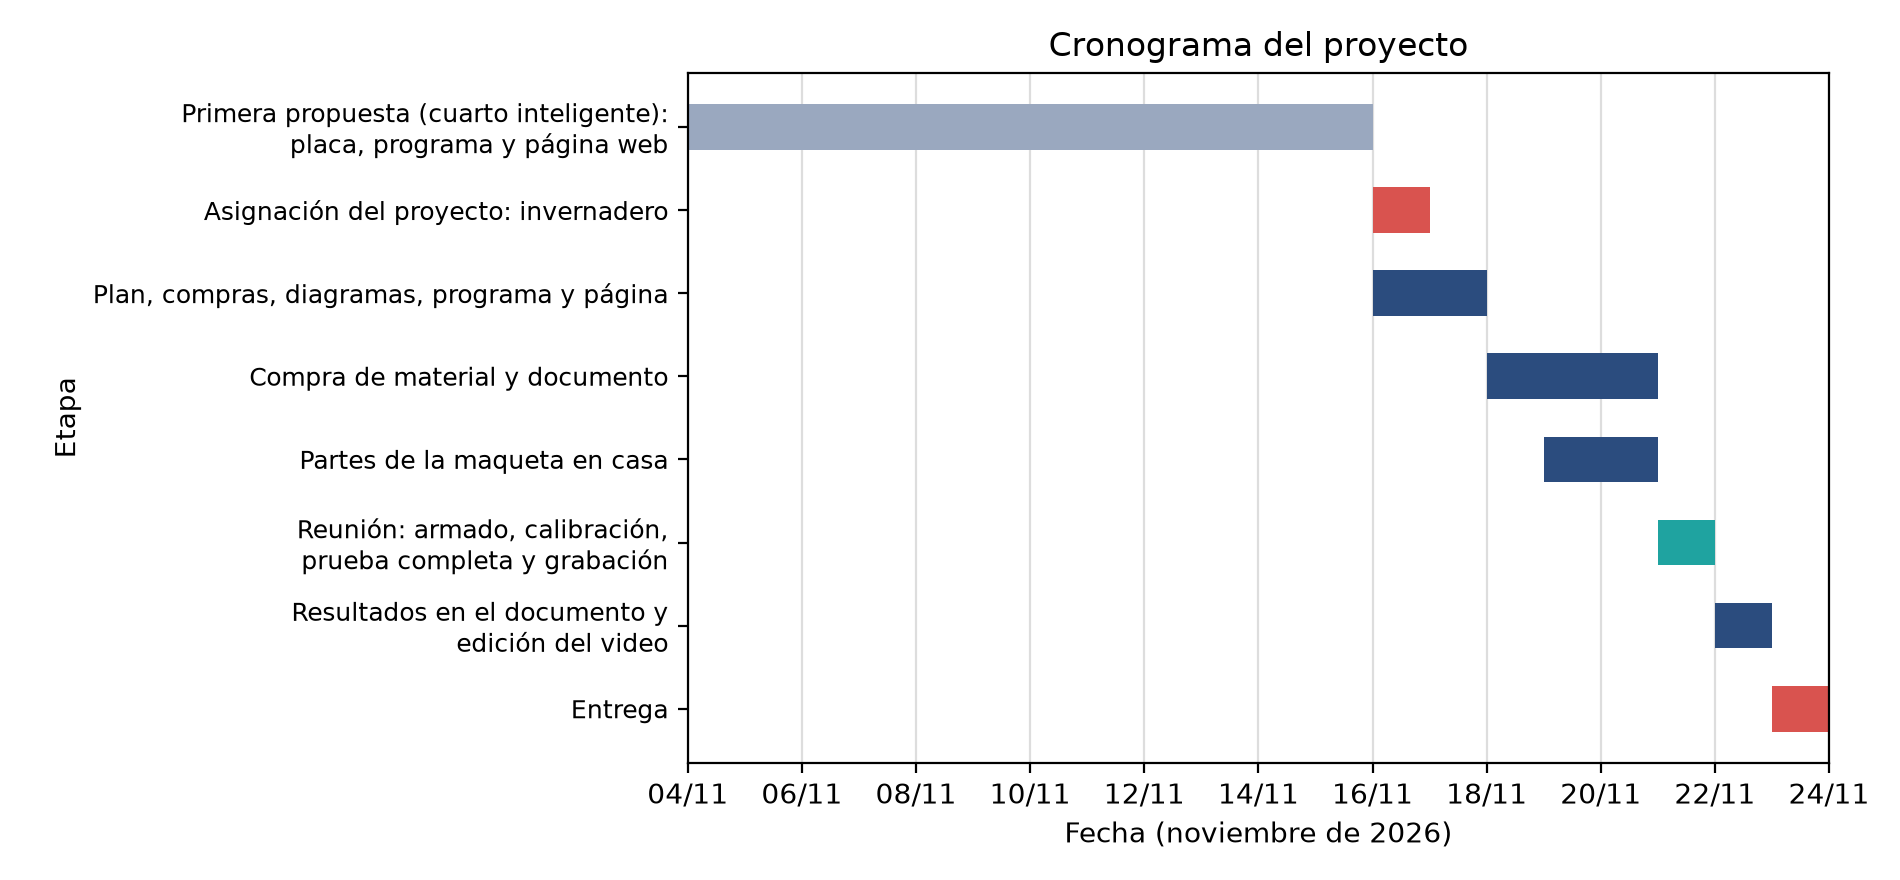
\includegraphics[width=\textwidth]{img/cronograma.png}
    \caption{Cronograma del proyecto.}
    \label{fig:cronograma}
\end{figure}

\newpage

% --- OBJETIVO ---
\section{Objetivo}

Mantener condiciones adecuadas dentro de un invernadero a escala mediante el monitoreo de la temperatura y de la
humedad de la tierra. Si la temperatura pasa de un límite, el sistema prende un ventilador y abre una ventana con un
servomotor, y si la tierra está seca riega por cierto tiempo con una bomba. Los datos de los sensores y el estado de
los actuadores se mandan por wifi y se grafican en tiempo real en el celular y en la computadora.

% --- MATERIAL ---
\section{Material}

\begin{table}[H]
\centering
\begin{tabularx}{\textwidth}{>{\raggedright\arraybackslash}p{0.45\textwidth}rX}
\toprule
\textbf{Pieza} & \textbf{Cant.} & \textbf{Uso} \\
\midrule
Tarjeta ESP32-S3-DevKitC-1 con módulo ESP32-S3-WROOM-1 N16R8 & 1 & Lee los sensores, controla los actuadores y sirve la página \\
Módulo DHT22 (AM2302) & 1 & Temperatura y humedad del aire \\
Sensor de humedad de suelo capacitivo v1.2 & 1 & Humedad de la tierra \\
Ventilador de \SI{5}{\volt}, $40 \times 40$~mm & 1 & Actuador 1: saca el aire caliente \\
Servomotor SG90 & 1 & Actuador 2: abre la ventana \\
Mini bomba de agua de diafragma de \SI{5}{\volt} & 1 & Actuador 3: riego \\
Transistor TIP120 & 2 & Interruptor del ventilador y de la bomba \\
Diodo 1N4007 & 2 & Protección contra el pico de voltaje de los motores \\
Resistencia de \SI{1}{\kilo\ohm} & 2 & Corriente de base de cada transistor \\
Capacitor electrolítico de \SI{1000}{\micro\farad} & 1 & Reserva de energía para el servo \\
Eliminador de \SI{5}{\volt}, \SI{2}{\ampere} con adaptador de jack & 1 & Alimentación de los actuadores \\
Protoboard de 830 puntos, jumpers y regleta de conexión & -- & Conexiones sin soldar \\
Cartón pluma, mica, tupper con tierra, planta y depósito de agua & -- & Maqueta \\
\bottomrule
\end{tabularx}
\caption{Material del proyecto.}
\end{table}

\newpage

% --- INTRODUCCIÓN ---
\section{Introducción}

El internet de las cosas consiste en conectar objetos de uso diario a una red para que midan algo de su entorno, manden
esos datos y, en algunos casos, actúen por su cuenta. Un sistema de este tipo se forma con tres partes: sensores que
convierten una variable física en una señal eléctrica, un procesador que interpreta esa señal y decide qué hacer, y un
enlace de comunicación que lleva la información hasta la persona que la consulta.

\subsection{Sensores y conversión analógica-digital}

La temperatura y la humedad son variables continuas, pero el procesador trabaja con números. El convertidor
analógico-digital toma muestras del voltaje de entrada y le asigna a cada una un número entero. Con $n$ bits hay $2^n$
niveles posibles, y el ESP32-S3 tiene convertidores de 12 bits (Espressif Systems, 2026), por lo que entrega valores de
0 a 4095. Cada nivel equivale a una fracción pequeña de la escala completa:
\[
2^{12} = 4096 \text{ niveles}, \qquad \frac{100\text{\%}}{4096} \approx 0.024\text{\% de la escala por nivel.}
\]
El sensor de temperatura DHT22 hace la conversión dentro de su propio encapsulado y manda la temperatura y la humedad
del aire ya en forma digital por un solo cable, con resolución de \SI{0.1}{\celsius} y exactitud de
$\pm$\SI{0.5}{\celsius} (\textit{Standard AM2302/DHT22}, s.f.). No admite más de una lectura cada dos segundos
(Adafruit, s.f.).

El sensor de humedad de la tierra es capacitivo. Dos pistas de cobre cubiertas forman un capacitor cuya capacitancia
depende de la constante dieléctrica de lo que lo rodea, y el agua la aumenta mucho. Como no mide la conductividad, sus
pistas no quedan expuestas al agua y no se corroen. Trabaja con 3.3 a \SI{5.5}{\volt} y su salida analógica va de 0 a
\SI{3.0}{\volt} (DFRobot, s.f.). El sensor no entrega un porcentaje: se calibra con una lectura al aire, que se toma
como tierra seca, y otra en agua, que se toma como saturada. Con esas dos lecturas, $L_s$ y $L_m$, la lectura $L$ se
pasa a porcentaje:
\[
h = 100\text{\%} \cdot \frac{L_s - L}{L_s - L_m}
\]

\subsection{Ruido y promedio de muestras}

Toda medición trae ruido, una variación aleatoria que se suma a la señal y que, como indica la capacidad de canal de
Shannon, limita cuánta información útil se puede obtener de ella. Cuando el ruido de cada muestra es independiente del
de las demás, al promediar $N$ muestras la señal se conserva y la desviación estándar del ruido baja en un factor
$\sqrt{N}$. Para las 16 muestras que promedia el programa en cada lectura del sensor de humedad:
\[
\sigma_{\text{prom}} = \frac{\sigma}{\sqrt{N}} = \frac{\sigma}{\sqrt{16}} = \frac{\sigma}{4},
\qquad 10\log_{10}(16) \approx 12\ \text{dB}
\]
El ruido queda en la cuarta parte y la relación señal a ruido en potencia mejora unos 12~dB. Un promedio así funciona
como un filtro pasabajas sencillo, porque deja pasar los cambios lentos de la humedad y atenúa las variaciones rápidas.

\subsection{Control con dos límites}

El ventilador y la ventana se controlan con un control de encendido y apagado. Si se usara un solo límite, una
temperatura que oscila alrededor de ese valor haría que el ventilador se prendiera y apagara en cada lectura. Por eso
se usan dos límites, uno para abrir y otro más bajo para cerrar; entre los dos el sistema conserva el estado que tenía.
A esta diferencia entre los dos límites se le llama histéresis.

El riego no puede seguir la misma regla, porque el agua tarda en llegar al sensor. Si la bomba siguiera prendida hasta
que el sensor marcara humedad, el tupper se inundaría. Por eso el riego se hace por pulsos: la bomba se prende unos
segundos, se espera a que el agua se absorba y se vuelve a medir.

\subsection{Actuadores: transistor, diodo y PWM}

Un pin de la placa entrega \SI{3.3}{\volt} con poca corriente, suficiente para dar una orden pero no para mover un
motor. El ventilador y la bomba se conectan a través de un transistor TIP120, que funciona como interruptor: una
corriente pequeña en la base deja pasar una corriente mucho mayor entre colector y emisor. El TIP120 es un Darlington,
dos transistores en cascada, con una ganancia de corriente mínima de 1000 y una corriente de colector de hasta
\SI{5}{\ampere} (onsemi, 2024). Con la resistencia de \SI{1}{\kilo\ohm} y el voltaje base-emisor máximo que da la hoja
de datos, \SI{2.5}{\volt}, la corriente de base en el peor caso es
\[
I_B = \frac{3.3\ \text{V} - 2.5\ \text{V}}{1\ \text{k}\Omega} = 0.8\ \text{mA},
\qquad I_C \leq h_{FE}\, I_B = 1000 \times 0.8\ \text{mA} = 0.8\ \text{A},
\]
lo que alcanza para el ventilador y la bomba.
\pendiente{anotar la corriente de la etiqueta o de la tienda del ventilador y de la bomba, y confirmar que es menor que 0.8 A}

Un motor guarda energía en el campo magnético de su bobina. Cuando el transistor lo apaga, la corriente no puede
desaparecer de golpe y el voltaje en la bobina crece hasta que encuentra por dónde descargarse, ya que
$v = L\,\frac{di}{dt}$. El diodo 1N4007 en paralelo con cada motor le da ese camino y protege al transistor. El TIP120
también trae un diodo interno entre colector y emisor (onsemi, 2024).

El servomotor no necesita transistor, porque la orden se le da con una señal de modulación por ancho de pulso, o PWM:
un pulso que se repite cada \SI{20}{\milli\second} y cuyo ancho indica el ángulo. Esa repetición equivale a una
frecuencia de
\[
f = \frac{1}{T} = \frac{1}{0.020\ \text{s}} = 50\ \text{Hz}.
\]
La placa genera la señal con un contador de 14 bits, así que divide el periodo en $2^{14} = 16384$ partes de
$20\,000\ \mu\text{s} / 16384 \approx 1.22\ \mu\text{s}$ cada una. El programa usa pulsos de \SI{500}{\micro\second}
para \ang{0} y de \SI{2400}{\micro\second} para \ang{180}; el ancho exacto para cada ángulo cambia de un servo a otro,
y por eso los ángulos de la ventana cerrada y abierta se ajustaron en la maqueta. Por ejemplo, para \ang{90}:
\[
t = 500\ \mu\text{s} + \frac{90^\circ}{180^\circ}\,(2400 - 500)\ \mu\text{s} = 1450\ \mu\text{s},
\qquad \frac{1450}{20\,000} \times 16\,383 \approx 1188 \text{ cuentas.}
\]

\subsection{Comunicación: wifi y HTTP}

La placa se comunica por wifi, que sigue el estándar IEEE 802.11. El ESP32-S3 trabaja en la banda de
\SI{2.4}{\giga\hertz} con las versiones b, g y n del estándar y con canales de 20 o \SI{40}{\mega\hertz} de ancho
(Espressif Systems, 2026). Por eso el hotspot del celular se configura en \SI{2.4}{\giga\hertz}, ya que una red solo
de \SI{5}{\giga\hertz} no admitiría a la placa. La página muestra la potencia de la señal que recibe la placa en dBm,
que es la potencia comparada con un milivatio en escala logarítmica:
\[
P_{\text{dBm}} = 10\log_{10}\frac{P}{1\ \text{mW}}, \qquad
-60\ \text{dBm} \;\Rightarrow\; P = 10^{-60/10}\ \text{mW} = 10^{-6}\ \text{mW} = 1\ \text{nW}
\]

La página de las gráficas se entrega con el modelo cliente-servidor. El servidor espera peticiones y el cliente las
hace; en este proyecto la placa es el servidor y el navegador del celular o de la computadora es el cliente. Se usa
HTTP, un protocolo de petición y respuesta sin estado en el que cada petición se atiende sin depender de las anteriores.
El cliente manda una petición con un método, como GET para pedir datos o POST para mandarlos, y una dirección, y el
servidor contesta con el contenido (Fielding et al., 2022).

En este proyecto se armó un invernadero a escala controlado por una ESP32-S3. La placa mide la temperatura con un DHT22
y la humedad de la tierra con un sensor capacitivo, controla un ventilador, un servo que abre una ventana y una bomba de
riego, y sirve una página web con los valores, las gráficas de los sensores y de los actuadores, y los ajustes del
sistema, que se consulta desde el celular y la computadora conectados a la misma red.

\newpage

% --- DESARROLLO ---
\section{Desarrollo}

\subsection{Descripción del sistema}

La figura~\ref{fig:bloques} muestra las partes del sistema. Los sensores mandan sus lecturas a la ESP32-S3, que cada
dos segundos decide el estado de los actuadores y guarda las lecturas en un historial. La misma placa atiende al
navegador del celular y de la computadora por wifi.

\begin{figure}[H]
    \centering
    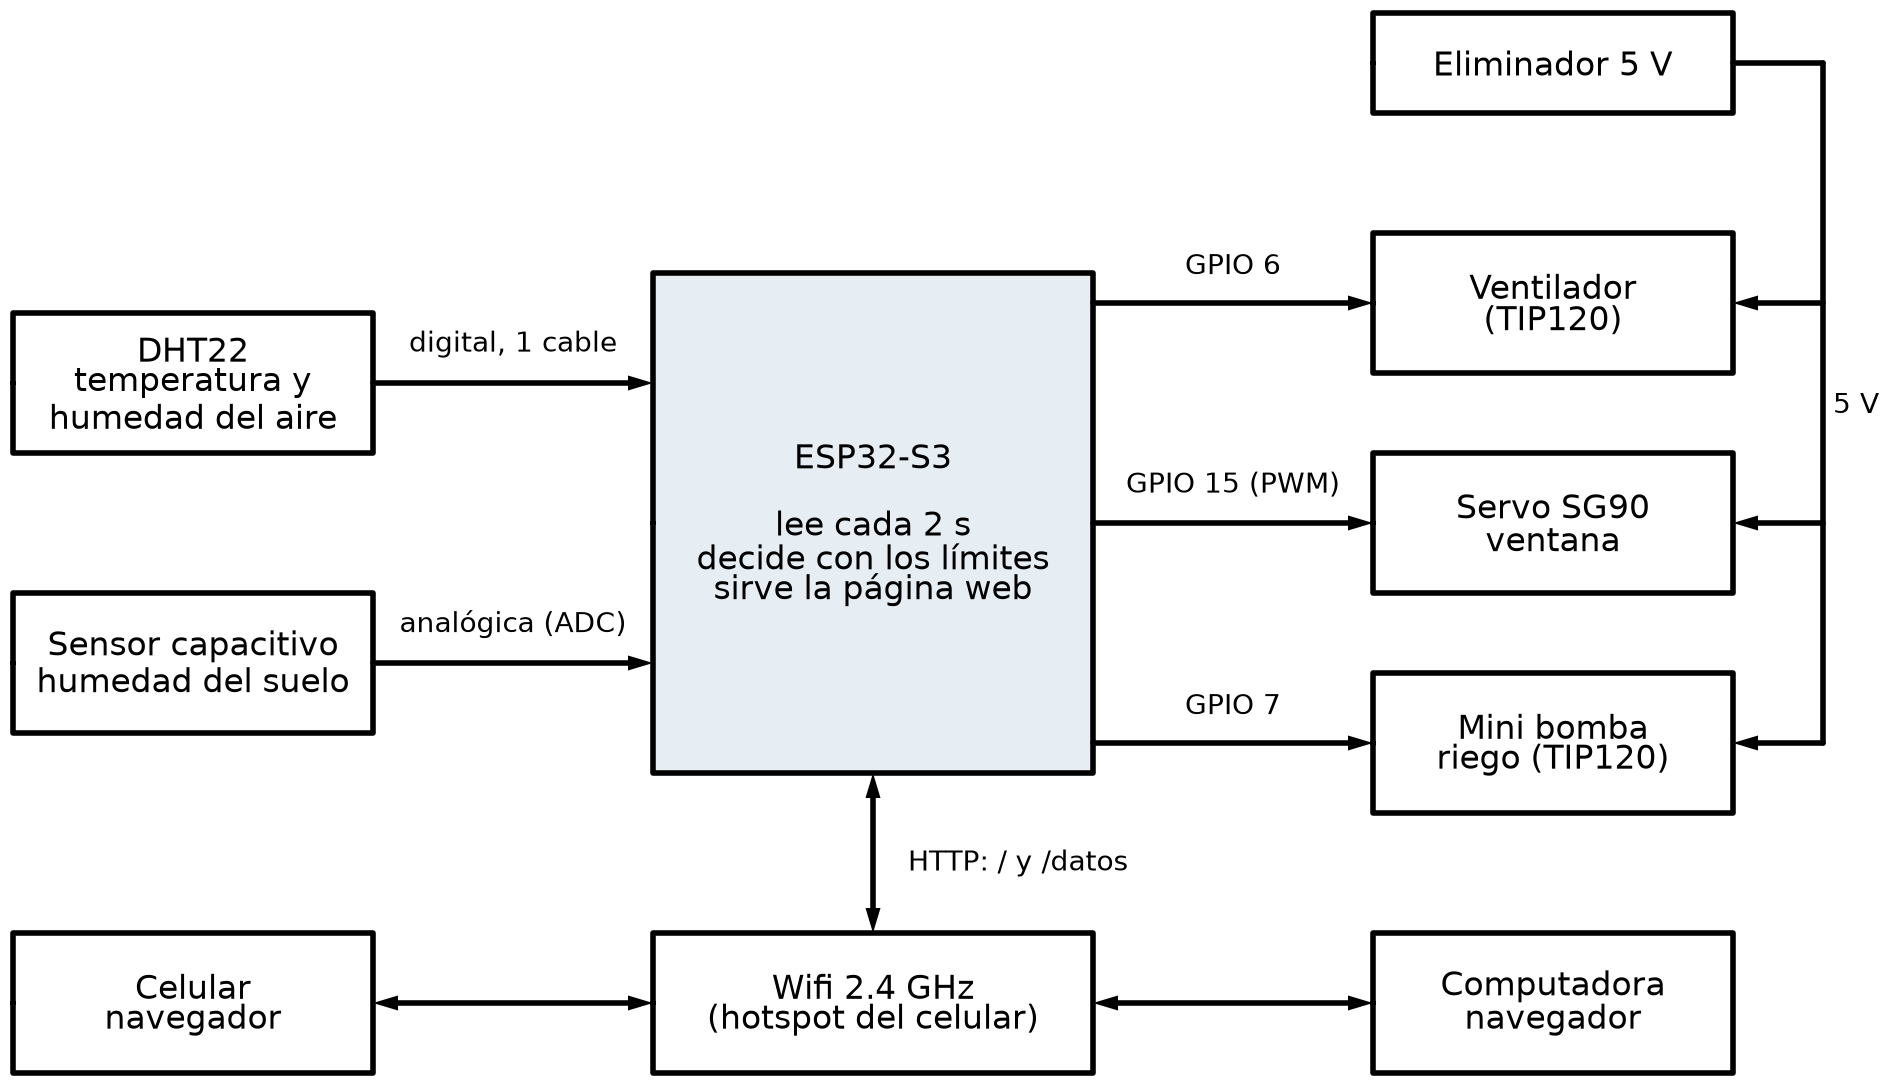
\includegraphics[width=0.95\textwidth]{img/diagrama_bloques.png}
    \caption{Diagrama de bloques del sistema.}
    \label{fig:bloques}
\end{figure}

\begin{table}[H]
\centering
\begin{tabularx}{\textwidth}{llX}
\toprule
\textbf{Pin} & \textbf{Conexión} & \textbf{Por qué ese pin} \\
\midrule
GPIO 4 & Dato del DHT22 & Digital; está del lado de la placa que queda libre en la protoboard \\
GPIO 5 & Salida del sensor de humedad & Pertenece al ADC1, que funciona aunque el wifi esté encendido \\
GPIO 6 & Base del TIP120 del ventilador & Salida digital \\
GPIO 7 & Base del TIP120 de la bomba & Salida digital \\
GPIO 15 & Señal del servo & Salida con PWM \\
\bottomrule
\end{tabularx}
\caption{Pines de la ESP32-S3. Todos están en la fila de pines J1 (Espressif Systems, s.f.-d).}
\label{tab:pines}
\end{table}

Los pines del 1 al 10 son los canales del ADC1, y del 11 en adelante pertenecen al ADC2 (Espressif Systems, s.f.-c),
que también lo usa el wifi (Espressif Systems, s.f.-a), así que el sensor de humedad va en un pin del ADC1. Los pines
35, 36 y 37 los ocupa la memoria PSRAM de esta versión del módulo (Espressif Systems, s.f.-d) y no se usan.

\subsection{Electrónica}

La figura~\ref{fig:esquema} muestra el esquema eléctrico por bloques. Los sensores se alimentan con los
\SI{3.3}{\volt} de la placa, de modo que sus salidas nunca pasan del voltaje que admiten los pines. Los tres actuadores
se alimentan con un eliminador de \SI{5}{\volt} aparte, porque los motores piden picos de corriente que harían
reiniciarse a la placa si se alimentaran de su puerto USB. Las tierras del eliminador y de la placa se unen, para que
las dos partes compartan la misma referencia de voltaje; sin esa unión, la señal de la placa no tendría un punto común
con el emisor de los transistores ni con el servo.

\begin{figure}[H]
    \centering
    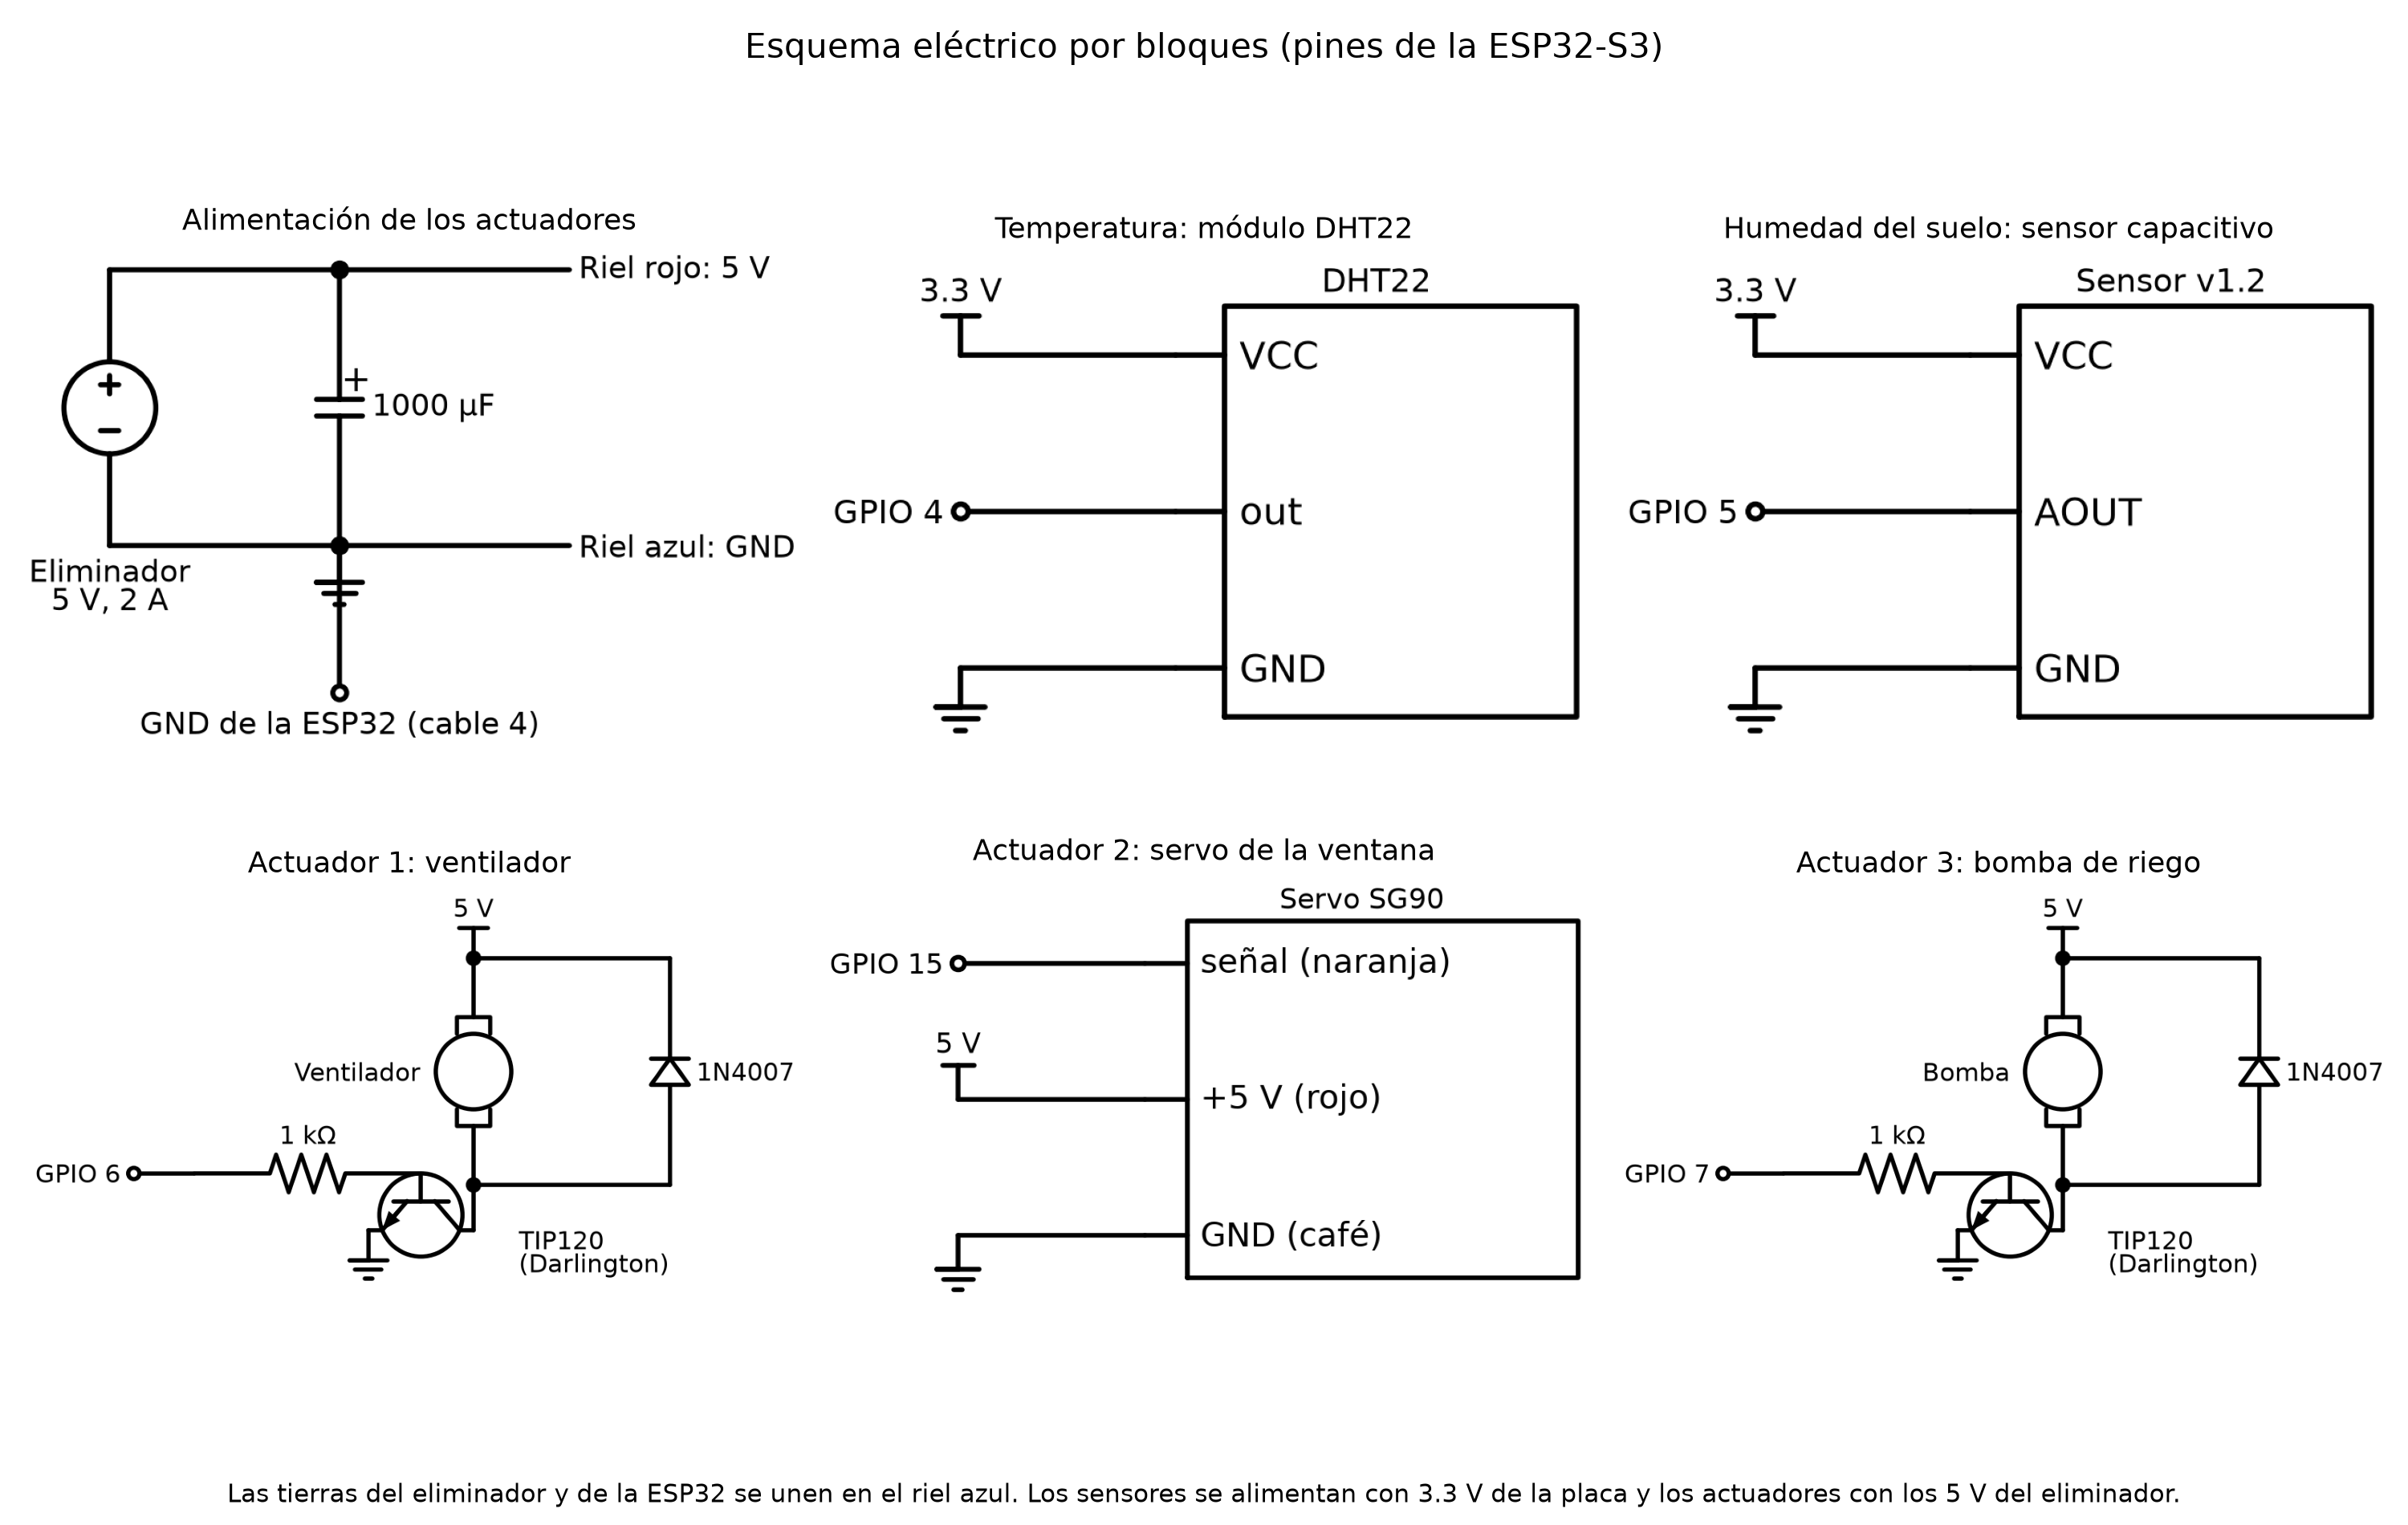
\includegraphics[width=\textwidth]{img/esquema_electrico.png}
    \caption{Esquema eléctrico por bloques.}
    \label{fig:esquema}
\end{figure}

El circuito se armó en una protoboard de 830 puntos. La placa queda montada sobre ella con la fila de pines J1 en la
columna i, de modo que cada pin tiene un hoyo libre en la columna j para su cable. La figura~\ref{fig:alambrado} muestra
el alambrado completo, con el número de cada cable; la lista de cables está en el anexo~\ref{anexo:cables}.

\begin{figure}[H]
    \centering
    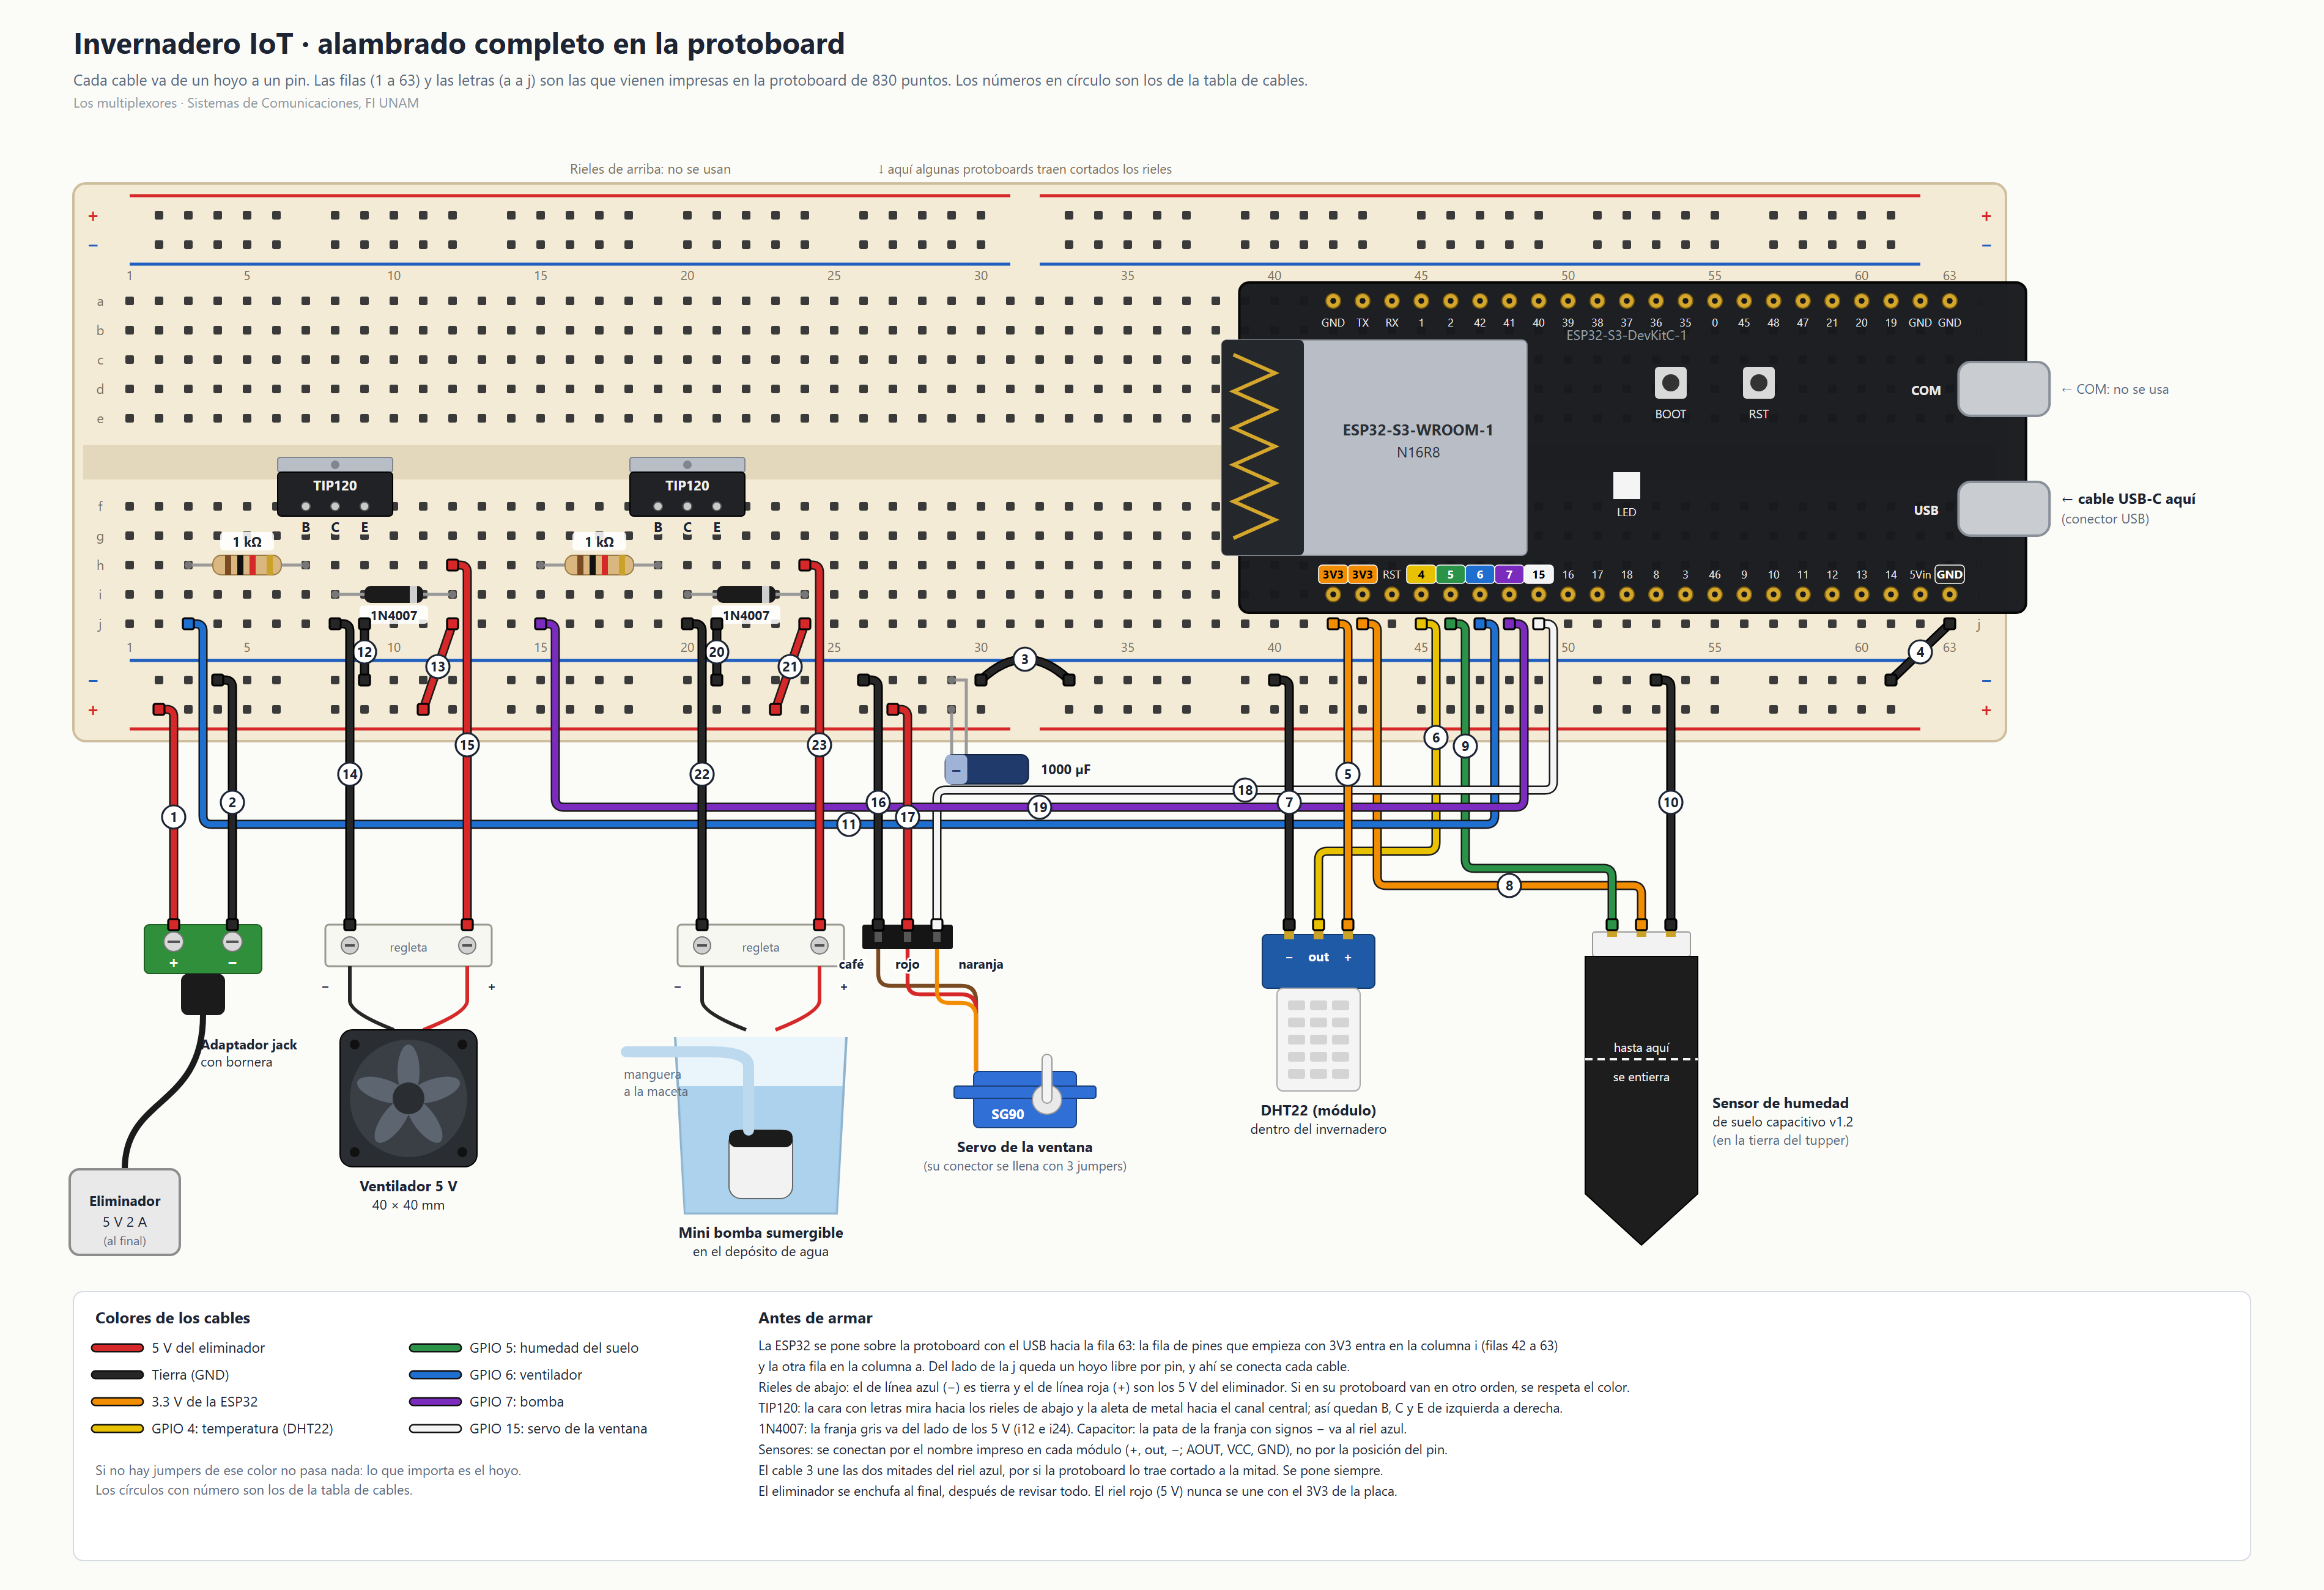
\includegraphics[width=\textwidth]{img/alambrado_completo.png}
    \caption{Alambrado sobre la protoboard. Las filas y las letras son las impresas en la protoboard.}
    \label{fig:alambrado}
\end{figure}

\subsection{Programa de la placa}

El programa está escrito en C++ con Arduino IDE y tiene dos archivos: la lógica en \texttt{invernadero.ino} y la página
web en \texttt{pagina.h}. La figura~\ref{fig:flujo} muestra el ciclo principal. En cada vuelta la placa atiende al
navegador; cada dos segundos lee los sensores y decide la ventilación, y en todas las vueltas revisa el riego, mueve la
ventana hacia su posición y revisa el wifi. Ninguna de estas tareas se queda esperando, así que la página responde
mientras la bomba riega o la ventana se mueve.

\begin{figure}[H]
    \centering
    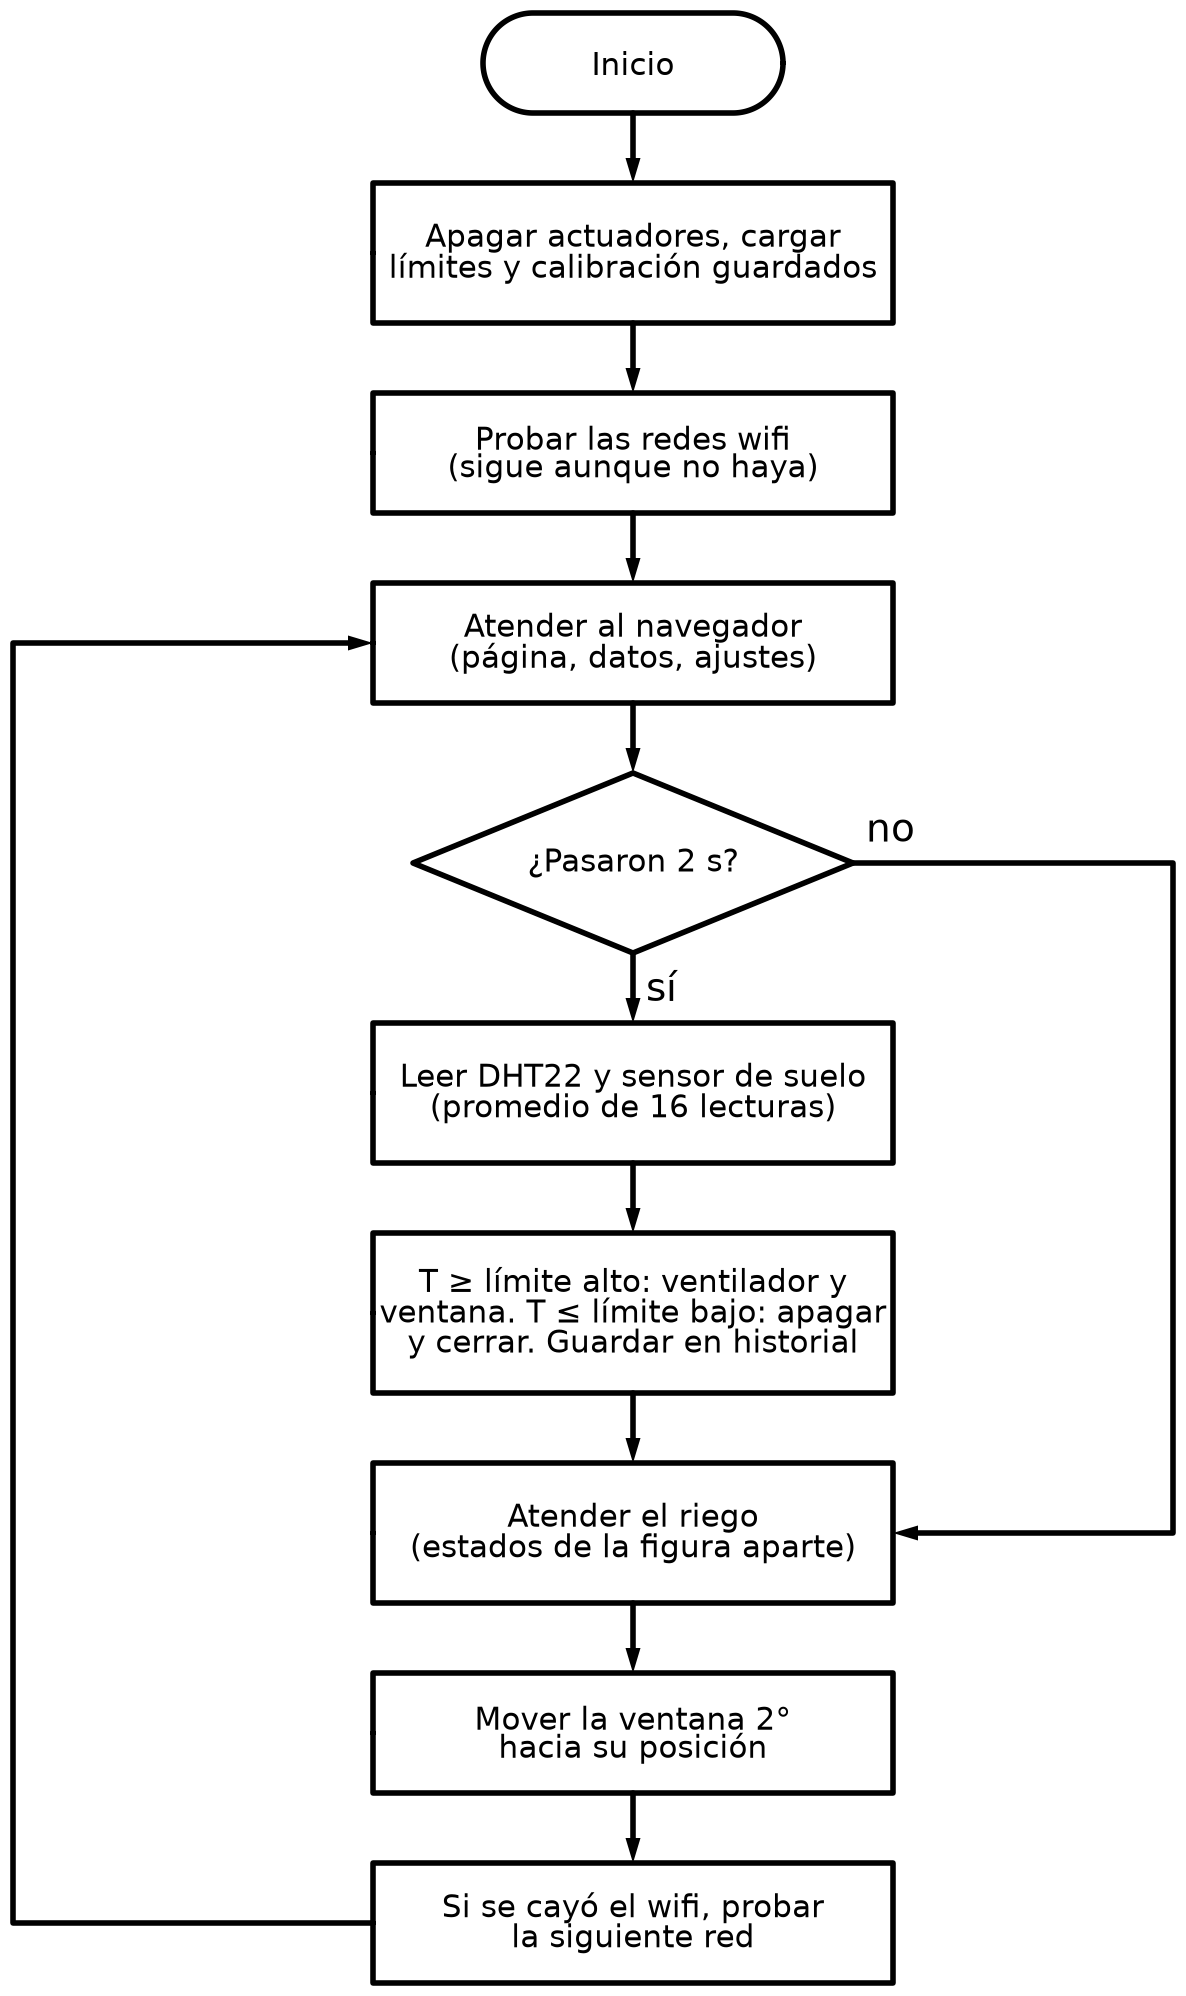
\includegraphics[height=0.62\textheight]{img/diagrama_flujo.png}
    \caption{Diagrama de flujo del ciclo principal del programa.}
    \label{fig:flujo}
\end{figure}

Las lecturas se toman cada dos segundos porque el DHT22 no admite más de una lectura en ese tiempo (Adafruit, s.f.).
El historial guarda 150 lecturas, que cubren cinco minutos:
\[
150 \times 2\ \text{s} = 300\ \text{s} = 5\ \text{min}
\]
El historial es circular, de modo que cada lectura nueva reemplaza a la más vieja cuando se llena. Si el DHT22 falla en
una lectura, el programa conserva el último valor bueno; si falla tres veces seguidas, marca la temperatura como sin
lectura, apaga el ventilador y cierra la ventana.

El riego se programó como una máquina de estados, que se muestra en la figura~\ref{fig:estados}. En el estado de
espera, si la humedad baja del límite, la bomba se prende y el sistema pasa a regar. Al cumplirse los segundos de
riego, la bomba se apaga y empieza la espera para que el agua se absorba. Al terminar, si la tierra ya tiene humedad,
regresa a esperar; si sigue seca, riega otra vez, y si ya regó tres veces seguidas se pausa. La pausa evita que se tire
agua cuando el sensor está fuera de la tierra o el depósito se vació, y se quita sola cuando la humedad vuelve o con un
botón de la página.

\begin{figure}[H]
    \centering
    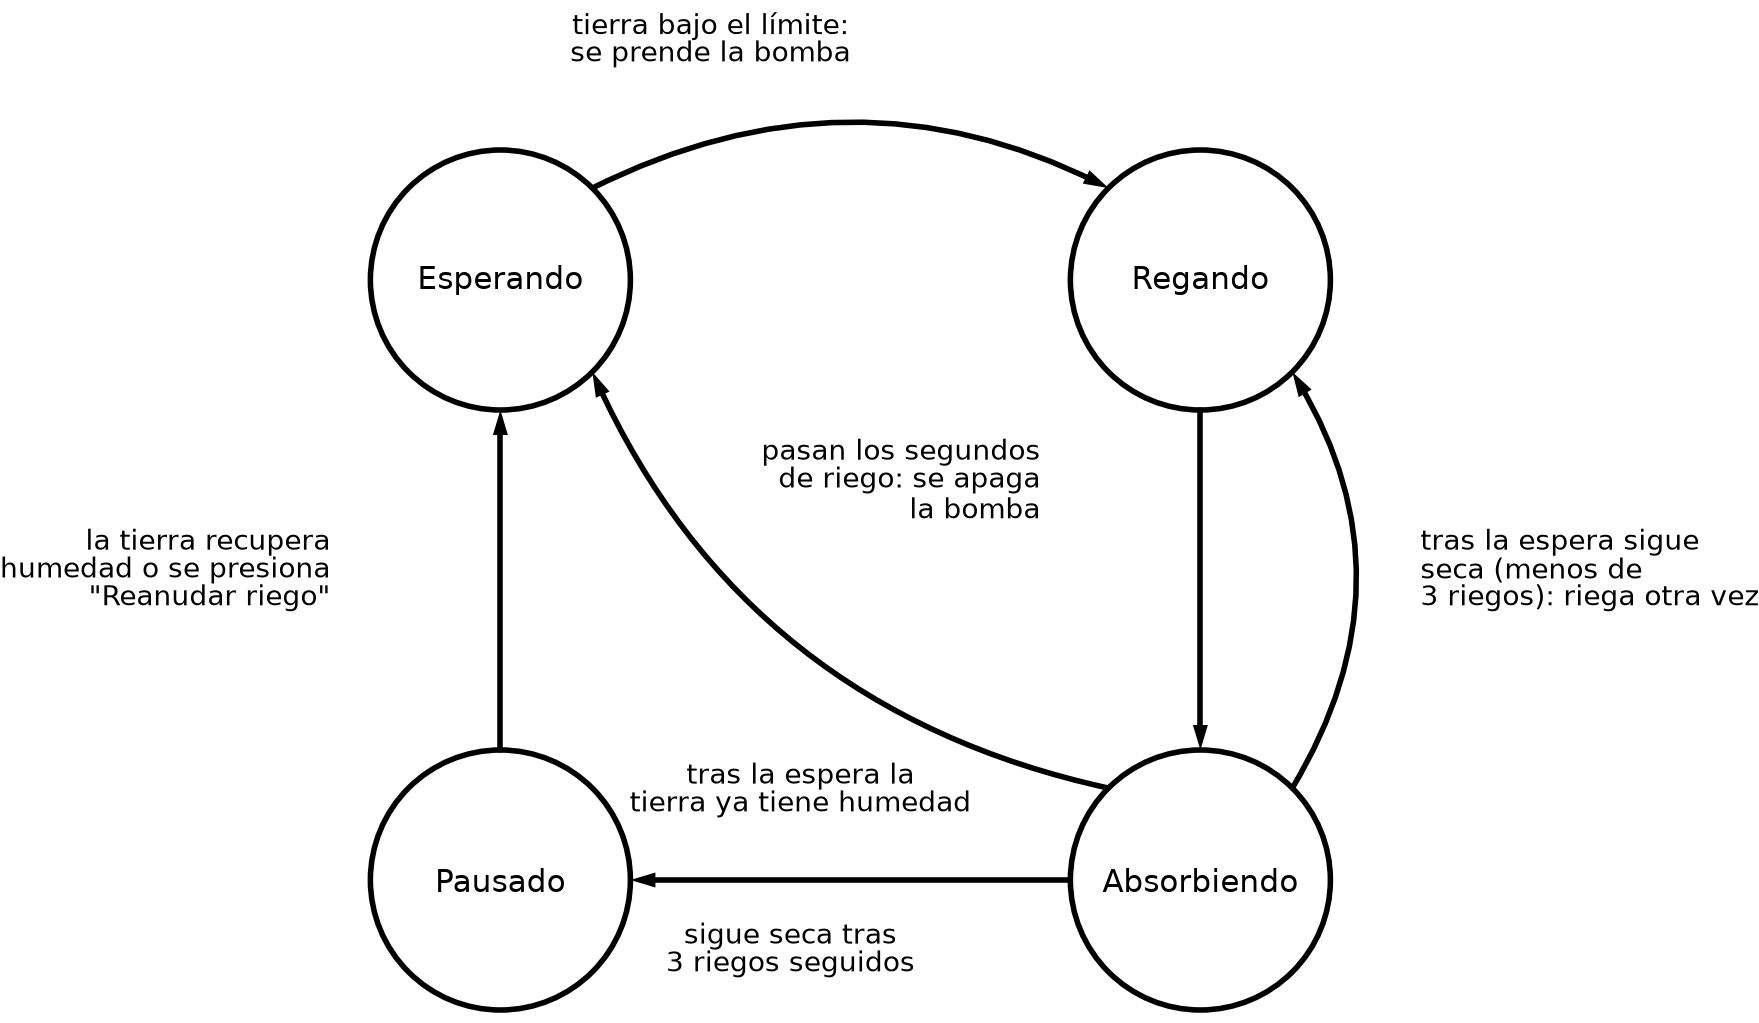
\includegraphics[width=0.85\textwidth]{img/estados_riego.png}
    \caption{Estados del riego.}
    \label{fig:estados}
\end{figure}

La ventana no salta de una posición a otra: el programa mueve el servo dos grados cada \SI{15}{\milli\second}, así que
recorre \ang{90} en unos
\[
\frac{90^\circ}{2^\circ} \times 15\ \text{ms} = 675\ \text{ms},
\]
lo que se ve suave en el video y evita que el servo pida toda su corriente de golpe.

La tabla~\ref{tab:ajustes} resume los ajustes. Se pueden cambiar desde la página, y la placa los guarda en su memoria
no volátil, de modo que se conservan aunque se desconecte.

\begin{table}[H]
\centering
\begin{tabularx}{\textwidth}{lrX}
\toprule
\textbf{Ajuste} & \textbf{De fábrica} & \textbf{Uso} \\
\midrule
Temperatura para abrir & \SI{28}{\celsius} & Prende el ventilador y abre la ventana \\
Temperatura para cerrar & \SI{26}{\celsius} & Apaga el ventilador y cierra la ventana \\
Humedad para regar & 35~\% & Por debajo de este valor se riega \\
Segundos de riego & \SI{2}{\second} & Tiempo que se prende la bomba en cada riego \\
Segundos de espera & \SI{15}{\second} & Tiempo para que el agua se absorba antes de volver a medir \\
Lectura al aire & 3000 & Calibración del sensor de humedad (tierra seca) \\
Lectura en agua & 1300 & Calibración del sensor de humedad (saturada) \\
\bottomrule
\end{tabularx}
\caption{Ajustes del sistema. Los valores que se usaron en la prueba están en la tabla~\ref{tab:calibracion}.}
\label{tab:ajustes}
\end{table}

Al prender, la placa prueba las redes wifi guardadas, una tras otra. Si ninguna aparece, sigue controlando los
actuadores sin wifi y vuelve a intentar cada doce segundos con la siguiente red. El LED de la tarjeta indica el estado:
parpadea en azul mientras se conecta, queda en verde con wifi y en rojo sin él. Cada vez que se conecta anuncia el
nombre \texttt{invernadero.local} en la red, para que la página se pueda abrir sin conocer su dirección IP, y además
escribe la IP en el monitor serie.

\subsection{Página web y conexión IoT}

La página está guardada en la memoria de la placa y no usa librerías ni tipos de letra de internet, para que funcione
con un hotspot sin datos. El navegador la pide una vez y después, cada dos segundos, pide los datos. La placa contesta
con un texto en formato JSON que trae las lecturas, el estado de los actuadores y del riego, los ajustes, la potencia de
la señal wifi y el historial de los últimos cinco minutos. La tabla~\ref{tab:rutas} resume las direcciones que atiende.

\begin{table}[H]
\centering
\begin{tabularx}{\textwidth}{llX}
\toprule
\textbf{Dirección} & \textbf{Método} & \textbf{Qué hace} \\
\midrule
\texttt{/} & GET & Entrega la página \\
\texttt{/datos} & GET & Lecturas, actuadores, ajustes e historial en JSON \\
\texttt{/ajustes} & POST & Guarda los límites y los tiempos de riego \\
\texttt{/calibrar} & POST & Guarda la lectura actual del sensor como seco o mojado \\
\texttt{/reanudar} & POST & Quita la pausa del riego \\
\texttt{/fabrica} & POST & Regresa los ajustes a los valores de fábrica \\
\bottomrule
\end{tabularx}
\caption{Direcciones que atiende el servidor de la placa.}
\label{tab:rutas}
\end{table}

La página tiene cuatro partes:
\begin{itemize}[label=$\bullet$]
    \item Un dibujo del invernadero visto de frente, con cada lectura escrita junto a su sensor. En el dibujo el
          ventilador gira, la ventana se abre y caen gotas cuando cada actuador está activo.
    \item Las gráficas de temperatura y de humedad de los últimos cinco minutos, con una franja que marca los límites,
          para que se vea por qué cambió cada actuador.
    \item Una gráfica de los actuadores con un carril para cada uno, que se llena cuando estuvo prendido o abierto.
    \item Un panel para cambiar los ajustes, calibrar el sensor y descargar las lecturas en un archivo CSV.
\end{itemize}
Las gráficas se dibujan en el propio navegador, y la misma página se acomoda al ancho de la pantalla del celular o de la
computadora. Si la placa deja de responder, la página avisa desde qué hora no hay datos y sigue intentando.

\figuraopcional{img/captura_computadora.png}{\textwidth}{Página en la computadora durante la prueba.}
\figuraopcional{img/captura_celular.png}{0.4\textwidth}{Página en el celular durante la prueba.}

\subsection{Maqueta}

La maqueta es un invernadero de cartón pluma con techo de mica sobre una base de $50 \times 35$~cm. La ventana está en
la pared izquierda y el servo hace de bisagra, sin varillas ni mecanismos. El ventilador está en la pared derecha,
del lado de la protoboard, para que sus cables sean cortos. Dentro van el tupper con tierra y una planta, el sensor de
humedad enterrado y el DHT22 en la pared trasera, lejos de la tierra mojada. El depósito de agua y la bomba están
afuera. La bomba es de diafragma, así que no se mete al agua: chupa del depósito por una manguera y empuja el agua
por otra, que entra por la pared trasera y queda acostada sobre la tierra, con el extremo tapado y unos hoyitos que
reparten el agua como una regadera. El frente es una hoja de mica que se levanta, para meter la mano y
para que se vea el interior. La figura~\ref{fig:maqueta} muestra el croquis con medidas.

\begin{figure}[H]
    \centering
    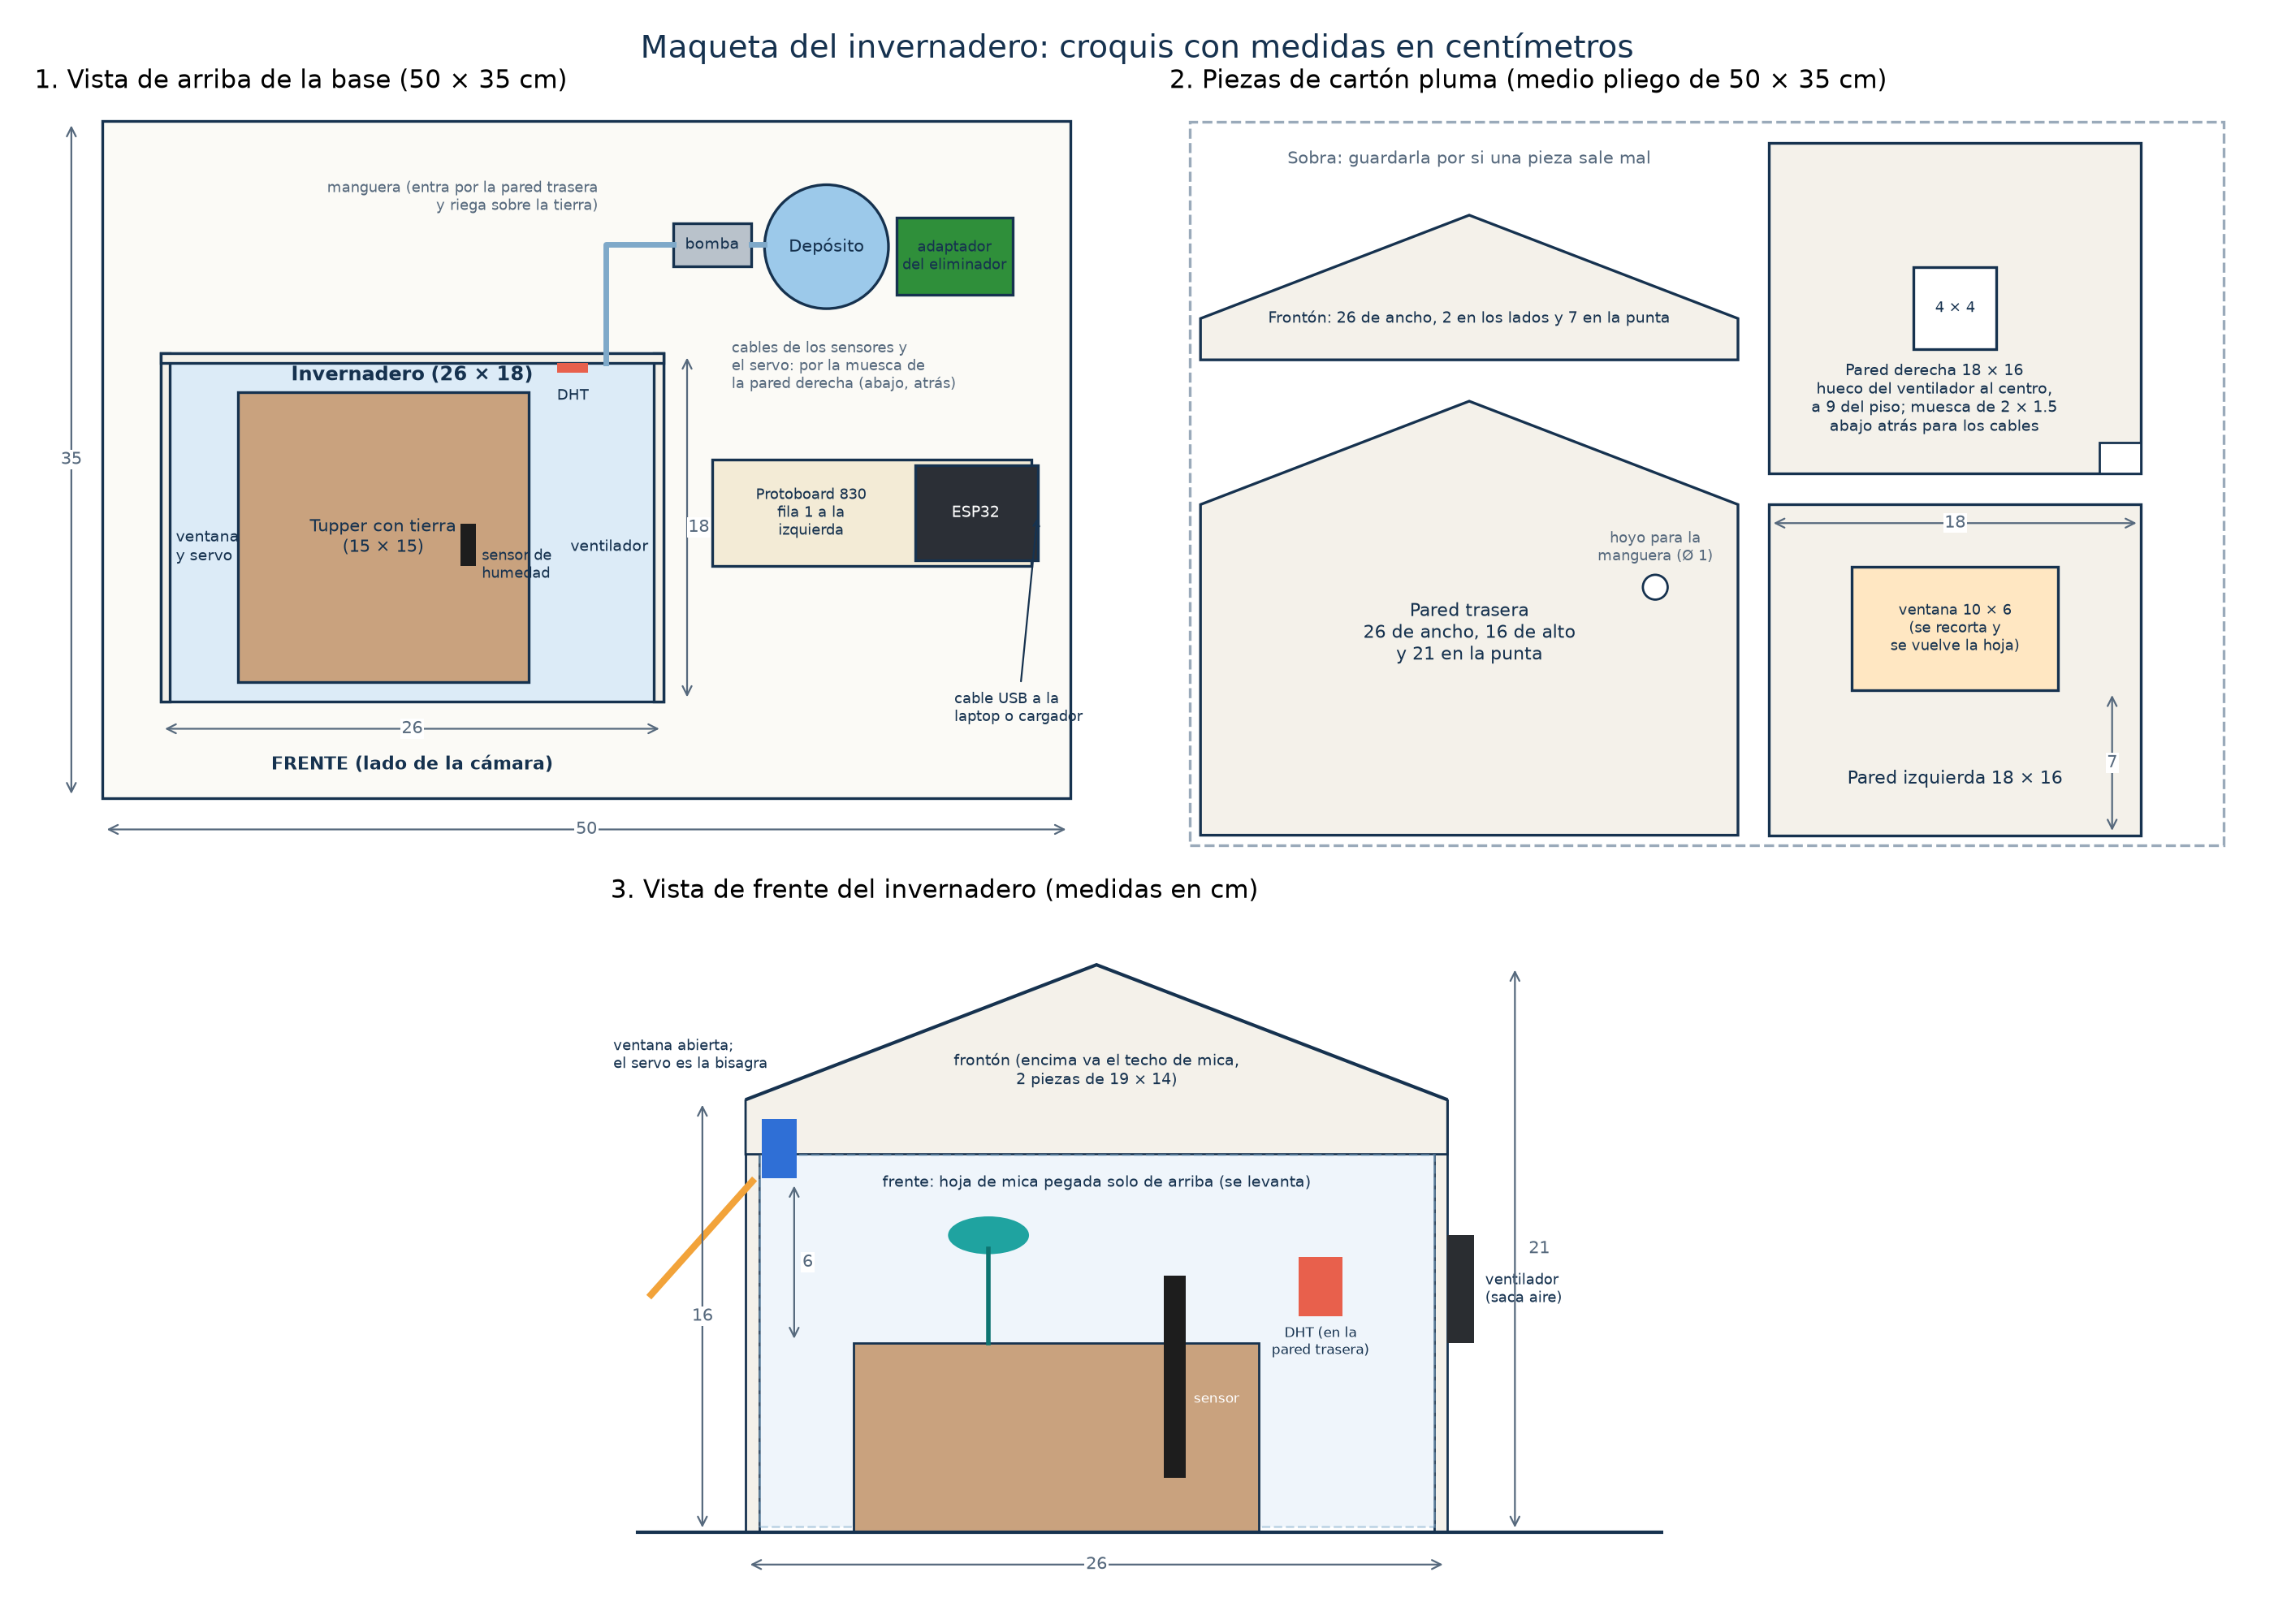
\includegraphics[width=\textwidth]{img/maqueta_croquis.png}
    \caption{Croquis de la maqueta, con medidas en centímetros.}
    \label{fig:maqueta}
\end{figure}

\figuraopcional{img/foto_maqueta.png}{0.8\textwidth}{Maqueta terminada.}
\figuraopcional{img/foto_protoboard.png}{0.8\textwidth}{Circuito armado en la protoboard.}

\newpage

% --- PRUEBAS Y RESULTADOS ---
\section{Pruebas y resultados}

\subsection{Calibración y ajustes}

\begin{table}[H]
\centering
\begin{tabularx}{\textwidth}{Xr}
\toprule
\textbf{Dato} & \textbf{Valor} \\
\midrule
Lectura del sensor de humedad al aire & \pendiente{} \\
Lectura del sensor de humedad en agua & \pendiente{} \\
Humedad de la tierra húmeda del tupper & \pendiente{} \\
Temperatura del lugar & \pendiente{} \\
Temperatura para abrir y para cerrar & \pendiente{} \\
Humedad para regar, segundos de riego y de espera & \pendiente{} \\
Agua de un riego, medida con un vaso graduado & \pendiente{} \\
Potencia de la señal wifi en la prueba & \pendiente{} \\
\bottomrule
\end{tabularx}
\caption{Calibración y ajustes que se usaron en la prueba.}
\label{tab:calibracion}
\end{table}

\pendiente{explicar en un párrafo cómo se eligieron los límites a partir de estos valores}

\subsection{Prueba completa}

La prueba se hizo con la placa, el celular y la computadora conectados al hotspot del celular en
\SI{2.4}{\giga\hertz}.

\begin{table}[H]
\centering
\begin{tabularx}{\textwidth}{Xl}
\toprule
\textbf{Prueba} & \textbf{Resultado} \\
\midrule
La página abre en el celular y en la computadora y se actualiza cada \SI{2}{\second} & \pendiente{} \\
Al calentar el DHT22 sobre el límite, el ventilador se prende y la ventana se abre & \pendiente{} \\
Al bajar al límite de cerrar, el ventilador se apaga y la ventana se cierra & \pendiente{} \\
Con el sensor fuera de la tierra, la bomba riega, espera y vuelve a medir & \pendiente{} \\
Tras tres riegos seguidos el riego se pausa y la página avisa & \pendiente{} \\
Con el sensor en la tierra húmeda, el riego se detiene & \pendiente{} \\
La gráfica de actuadores muestra cada activación & \pendiente{} \\
La placa se reconecta sola al apagar y prender el hotspot & \pendiente{} \\
Los ajustes se conservan al desconectar la placa & \pendiente{} \\
\bottomrule
\end{tabularx}
\caption{Resultados de la prueba completa.}
\end{table}

\subsection{Lecturas durante la prueba}

Las gráficas siguientes se hicieron con el archivo CSV que se descargó de la página al final de la prueba.

\figuraopcional{img/resultados_temperatura.png}{\textwidth}{Temperatura y estado de la ventilación durante la prueba.}
\figuraopcional{img/resultados_humedad.png}{\textwidth}{Humedad del suelo y riegos durante la prueba.}

\pendiente{describir lo que se ve en las gráficas: cuándo se activó cada actuador y con qué lectura}

\newpage

% --- CONCLUSIONES ---
\section{Conclusiones}

\pendiente{escribir con los resultados de la prueba; si el profesor pide conclusiones individuales, cada integrante
escribe la suya}

\newpage

% --- BIBLIOGRAFÍA ---
% Solo fuentes verificadas en Proyecto/02_Investigacion/fuentes.md
\section*{Bibliografía}
\addcontentsline{toc}{section}{Bibliografía}
\begin{list}{}{\setlength{\leftmargin}{1.27cm}\setlength{\itemindent}{-1.27cm}\setlength{\itemsep}{4pt}}
\item Adafruit. (s.f.). \textit{DHT11, DHT22 and AM2302 sensors: Overview}. Adafruit Learning System.
    \url{https://learn.adafruit.com/dht/overview}
\item DFRobot. (s.f.). \textit{Gravity: Analog capacitive corrosion resistant soil moisture sensor} (SEN0193).
    DFRobot Wiki. \url{https://wiki.dfrobot.com/Capacitive_Soil_Moisture_Sensor_SKU_SEN0193}
\item Espressif Systems. (2026). \textit{ESP32-S3 series datasheet} (Versión 2.2).
    \url{https://www.espressif.com/sites/default/files/documentation/esp32-s3_datasheet_en.pdf}
\item Espressif Systems. (s.f.-a). \textit{Analog to digital converter (ADC) oneshot mode driver: ESP32-S3}.
    ESP-IDF Programming Guide.
    \url{https://docs.espressif.com/projects/esp-idf/en/latest/esp32s3/api-reference/peripherals/adc/adc_oneshot.html}
\item Espressif Systems. (s.f.-b). \textit{ESP32-S3-WROOM-1 \& ESP32-S3-WROOM-1U datasheet} (Versión 1.8).
    \url{https://www.espressif.com/sites/default/files/documentation/esp32-s3-wroom-1_wroom-1u_datasheet_en.pdf}
\item Espressif Systems. (s.f.-c). \textit{GPIO \& RTC GPIO: ESP32-S3}. ESP-IDF Programming Guide.
    \url{https://docs.espressif.com/projects/esp-idf/en/latest/esp32s3/api-reference/peripherals/gpio.html}
\item Espressif Systems. (s.f.-d). \textit{ESP32-S3-DevKitC-1 v1.1: User guide}. ESP-DevKits documentation.
    \url{https://docs.espressif.com/projects/esp-dev-kits/en/latest/esp32s3/esp32-s3-devkitc-1/user_guide_v1.1.html}
\item Fielding, R., Nottingham, M., y Reschke, J. (Eds.). (2022). \textit{HTTP semantics} (RFC 9110).
    Internet Engineering Task Force. \url{https://www.rfc-editor.org/rfc/rfc9110.html}
\item onsemi. (2024). \textit{TIP120, TIP121, TIP122 (NPN); TIP125, TIP126, TIP127 (PNP): Plastic medium-power
    complementary silicon transistors} (Rev. 10) [Hoja de datos]. \url{https://www.onsemi.com/pdf/datasheet/tip120-d.pdf}
\item \textit{Standard AM2302/DHT22} [Hoja de datos]. (s.f.). Adafruit.
    \url{https://cdn-shop.adafruit.com/datasheets/Digital+humidity+and+temperature+sensor+AM2302.pdf}
\end{list}

\newpage
\appendix

% --- ANEXOS ---
\section{Piezas y cables de la protoboard}
\label{anexo:cables}

Las tablas salen del mismo script que dibuja el diagrama de alambrado, \texttt{alambrado.py}, que está en la carpeta
\texttt{documento/graficas} del repositorio.

\begin{longtable}{p{0.33\textwidth}p{0.6\textwidth}}
\toprule
\textbf{Pieza} & \textbf{Dónde va} \\
\midrule
\endhead
\entrada{tablas/piezas.tex}
\bottomrule
\end{longtable}

\begin{longtable}{rlp{0.36\textwidth}p{0.36\textwidth}}
\toprule
\textbf{\#} & \textbf{Color} & \textbf{Desde} & \textbf{Hasta} \\
\midrule
\endhead
\entrada{tablas/cables.tex}
\bottomrule
\end{longtable}

\section{Programa de la placa}

Programa principal (\texttt{firmware/invernadero\_dht22/invernadero\_dht22.ino}). La versión para el DHT11, en
\texttt{firmware/invernadero\_dht11}, solo cambia en el modelo del sensor. La página web, en \texttt{pagina.h}, está en el
repositorio del proyecto.

\lstinputlisting{../firmware/invernadero_dht22/invernadero_dht22.ino}

\end{document}
